\documentclass[journal,12pt,twocolumn]{IEEEtran}

\usepackage{setspace}
\usepackage{gensymb}

\singlespacing


\usepackage[cmex10]{amsmath}

\usepackage{amsthm}

\usepackage{mathrsfs}
\usepackage{txfonts}
\usepackage{stfloats}
\usepackage{bm}
\usepackage{cite}
\usepackage{cases}
\usepackage{subfig}

\usepackage{longtable}
\usepackage{multirow}

\usepackage{enumitem}
\usepackage{mathtools}
\usepackage{steinmetz}
\usepackage{tikz}
\usepackage{circuitikz}
\usepackage{verbatim}
\usepackage{tfrupee}
\usepackage[breaklinks=true]{hyperref}
\usepackage{graphicx}
\usepackage{tkz-euclide}
\usepackage{float}

\usetikzlibrary{calc,math}
\usepackage{listings}
    \usepackage{color}                                            %%
    \usepackage{array}                                            %%
    \usepackage{longtable}                                        %%
    \usepackage{calc}                                             %%
    \usepackage{multirow}                                         %%
    \usepackage{hhline}                                           %%
    \usepackage{ifthen}                                           %%
    \usepackage{lscape}     
\usepackage{multicol}
\usepackage{chngcntr}

\DeclareMathOperator*{\Res}{Res}

\renewcommand\thesection{\arabic{section}}
\renewcommand\thesubsection{\thesection.\arabic{subsection}}
\renewcommand\thesubsubsection{\thesubsection.\arabic{subsubsection}}

\renewcommand\thesectiondis{\arabic{section}}
\renewcommand\thesubsectiondis{\thesectiondis.\arabic{subsection}}
\renewcommand\thesubsubsectiondis{\thesubsectiondis.\arabic{subsubsection}}


\hyphenation{op-tical net-works semi-conduc-tor}
\def\inputGnumericTable{}                                 %%

\lstset{
%language=C,
frame=single, 
breaklines=true,
columns=fullflexible
}
\begin{document}
\newtheorem{theorem}{Theorem}[section]
\newtheorem{problem}{Problem}
\newtheorem{proposition}{Proposition}[section]
\newtheorem{lemma}{Lemma}[section]
\newtheorem{corollary}[theorem]{Corollary}
\newtheorem{example}{Example}[section]
\newtheorem{definition}[problem]{Definition}

\newcommand{\BEQA}{\begin{eqnarray}}
\newcommand{\EEQA}{\end{eqnarray}}
\newcommand{\define}{\stackrel{\triangle}{=}}
\bibliographystyle{IEEEtran}
\providecommand{\mbf}{\mathbf}
\providecommand{\pr}[1]{\ensuremath{\Pr\left(#1\right)}}
\providecommand{\qfunc}[1]{\ensuremath{Q\left(#1\right)}}
\providecommand{\sbrak}[1]{\ensuremath{{}\left[#1\right]}}
\providecommand{\lsbrak}[1]{\ensuremath{{}\left[#1\right.}}
\providecommand{\rsbrak}[1]{\ensuremath{{}\left.#1\right]}}
\providecommand{\brak}[1]{\ensuremath{\left(#1\right)}}
\providecommand{\lbrak}[1]{\ensuremath{\left(#1\right.}}
\providecommand{\rbrak}[1]{\ensuremath{\left.#1\right)}}
\providecommand{\cbrak}[1]{\ensuremath{\left\{#1\right\}}}
\providecommand{\lcbrak}[1]{\ensuremath{\left\{#1\right.}}
\providecommand{\rcbrak}[1]{\ensuremath{\left.#1\right\}}}
\theoremstyle{remark}
\newtheorem{rem}{Remark}
\newcommand{\sgn}{\mathop{\mathrm{sgn}}}
\providecommand{\abs}[1]{\left\vert#1\right\vert}
\providecommand{\res}[1]{\Res\displaylimits_{#1}} 
\providecommand{\norm}[1]{\left\lVert#1\right\rVert}
%\providecommand{\norm}[1]{\lVert#1\rVert}
\providecommand{\mtx}[1]{\mathbf{#1}}
\providecommand{\mean}[1]{E\left[ #1 \right]}
\providecommand{\fourier}{\overset{\mathcal{F}}{ \rightleftharpoons}}
%\providecommand{\hilbert}{\overset{\mathcal{H}}{ \rightleftharpoons}}
\providecommand{\system}{\overset{\mathcal{H}}{ \longleftrightarrow}}
	%\newcommand{\solution}[2]{\textbf{Solution:}{#1}}
\newcommand{\solution}{\noindent \textbf{Solution: }}
\newcommand{\cosec}{\,\text{cosec}\,}
\providecommand{\dec}[2]{\ensuremath{\overset{#1}{\underset{#2}{\gtrless}}}}
\newcommand{\myvec}[1]{\ensuremath{\begin{pmatrix}#1\end{pmatrix}}}
\newcommand{\mydet}[1]{\ensuremath{\begin{vmatrix}#1\end{vmatrix}}}
\numberwithin{equation}{subsection}
\makeatletter
\@addtoreset{figure}{problem}
\makeatother
\let\StandardTheFigure\thefigure
\let\vec\mathbf
\renewcommand{\thefigure}{\theproblem}
\def\putbox#1#2#3{\makebox[0in][l]{\makebox[#1][l]{}\raisebox{\baselineskip}[0in][0in]{\raisebox{#2}[0in][0in]{#3}}}}
     \def\rightbox#1{\makebox[0in][r]{#1}}
     \def\centbox#1{\makebox[0in]{#1}}
     \def\topbox#1{\raisebox{-\baselineskip}[0in][0in]{#1}}
     \def\midbox#1{\raisebox{-0.5\baselineskip}[0in][0in]{#1}}
\vspace{3cm}
\title{ASSIGNMENT 5}
\author{Atla keerthana}
\maketitle
\newpage
\bigskip
\renewcommand{\thefigure}{\theenumi}
\renewcommand{\thetable}{\theenumi}
Download all python codes from 
\begin{lstlisting}
https://github.com/BatharajuRamana/Assignment2/tree/main/Assignment2/codes
\end{lstlisting}
%
and latex-tikz codes from 
%
\begin{lstlisting}
https://github.com/BatharajuRamana/Assignment2/tree/main/Assignment2/main.tex
\end{lstlisting}
%
\section{Question No 2.23(Quad forms)}
Find the roots of the following quadratic equations, if they exit.
%
\begin{enumerate}
%\begin{multicols}{2}
\item
\begin{align}
\begin{split}
3x^2-5x+2&=0 \label{1.0.1}
\end{split}
\end{align}
\item
\begin{align}
\begin{split}
x^2+4x+5&=0 \label{1.0.2}
\end{split}
\end{align}
%\end{multicols}
\end{enumerate}
%
\section{SOLUTION}  
\begin{enumerate}
\item
The vector form of
\begin{align}
y&=3x^2-5x+2
\end{align}
is
\begin{align}
\vec{x}^T \myvec{3 & 0\\0 & 0}\vec{x}+ \myvec{-5 & 0}\vec{x}+2=0
\end{align}
Thus
\begin{align}
y=0\implies3x^2-5x+2 &=0
\end{align}
%
Compare given quadratic equation  $3x ^2 -5x +2 = 0$ with $ax^2 + bx + c = 0$,we get
\begin{align}
a=3,b&=-5,c=2
\end{align}
so,
\begin{align}
b^2-4ac&=(-5)^2-4(3)(2)\\
&=25-24=1>0
\end{align}
Since the square of a real number is positive. 
\begin{align}
 (x-1)(3x-2) &=0 \\
 x=1, \frac{2}{3}
\end{align}
The roots are 1 and 0.66
\begin{align}
 x=\myvec{1\\0},\myvec{0.66\\0} 
\end{align}
%
which can be verified from the fig\eqref{1.0.1} generated by following python code.
%
\numberwithin{figure}{section}
\begin{figure}[ht!]
Plot of \eqref{1.0.1} -
    \centering
    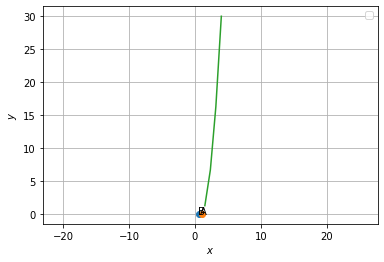
\includegraphics[width=\columnwidth]{figure5.png}
    \caption{roots of $3x^2-5x+2$.}
    \label{fig:Roots Of $3x^2-5x+2 &=$.}
\end{figure} 
\item
The vector form of
\begin{align}
y&=x^2+4x+5
\end{align}
is
\begin{align}
\vec{x}^T \myvec{1 & 0\\0 & 0}\vec{x}+ \myvec{4 & 0}\vec{x}+5=0
\end{align}
Thus
\begin{align}
y=0\implies x^2+4x+5 &=0
\end{align}
%
Compare given quadratic equation  $x ^2 +4x +5 = 0$ with $ax^2 + bx + c = 0$,we get
\begin{align}
a=1,b&=4,c=5
\end{align}
so,
\begin{align}
b^2-4ac&=(4)^2-4(1)(5)\\
&=16-20=-4<0
\end{align}
Since the square of a real number cannot be negative.so there are no real roots for the given equation.
\end{enumerate}
\end{document}